\part{Analyse et Conception }
\label{part:analyse-et-conception}
\chapter{Etude préliminaire et Méthode}

Dans ce chapitre, nous allons présenter l’étude préliminaire de notre projet de
création collaborative et de partage d’arbres généalogiques, ainsi que la
méthodologie que nous allons suivre pour sa conception et son développement.
Nous commencerons par une analyse approfondie de l’existant. Nous décrirons la
situation actuelle de \firm dans le domaine de la généalogie en ligne, nous
identifierons ses limites et nous proposerons des solutions pour les surmonter.

Ensuite, nous présenterons la méthode que nous allons utiliser pour concevoir notre
plateforme. Nous mettrons l’accent sur le langage de modélisation \ac{UML} ,
ainsi que sur les différents types de diagrammes UML que nous utiliserons pour
représenter notre système de manière visuelle et structurée. Nous discuterons
également des processus de développement que nous allons adopter, notamment
le \ac{UP} et le \ac{2TUP}. Nous verrons comment ils peuvent être intégrés
à UML pour assurer une gestion efficace du projet.

Ce chapitre posera les bases nécessaires à la réalisation de notre projet en
fournissant une compréhension approfondie de son contexte et en établissant
les lignes directrices pour sa conception et son développement. En combinant
une analyse approfondie de l’existant avec une méthodologie de conception
rigoureuse, nous sommes bien placés pour créer une plateforme généalogique
collaborative et innovante qui répondra aux besoins de nos utilisateurs tout
en garantissant sa robustesse et sa pérennité.

\section{Etude de l'existant}
\subsection{Description des activités (la situation actuelle)}
Actuellement, \firm ne dispose pas d’une plateforme dédiée à la création
collaborative et au partage d’arbres généalogiques. Les activités liées à la
généalogie sont principalement effectuées de manière traditionnelle, impliquant
la collecte de documents papier, la communication verbale et l’échange de fichiers
numériques par courrier électronique ou d’autres moyens non structurés. Les
membres de la famille rencontrent souvent des difficultés pour collaborer
efficacement à la création et au partage d'arbres généalogiques en raison de
l'absence d'un outil centralisé et convivial.

\subsection{Critique de l'existant (les limites)}
Cette approche traditionnelle présente plusieurs limites. Elle rend difficile
la collaboration entre les membres de la famille, en particulier ceux qui sont
éloignés géographiquement, et ne permet pas un partage facile et sécurisé des
informations généalogiques. De plus, la préservation à long terme de l’histoire
familiale est compromise, car les documents papier peuvent se perdre ou se
détériorer avec le temps, et les fichiers numériques peuvent être dispersés et mal organisés.

\subsection{Proposition de solutions}
Pour surmonter ces défis, nous proposons les solutions suivantes :
\begin{itemize}
  \item  Utiliser des logiciels de généalogie hors ligne : cette solution implique
    l’installation de logiciels sur des ordinateurs personnels pour créer et gérer
    des arbres généalogiques. Cependant, cela peut présenter certaines limites
    en termes de collaboration et de partage, car les données sont souvent stockées
    localement et ne permettent pas une collaboration facile entre les membres de la famille.

  \item  Utiliser des sites web de généalogie : cela consiste à
    utiliser des sites web spécialisés en généalogie pour créer et partager des arbres
    généalogiques. Cette méthode est pratique, car elle permet de partager ses arbres
    avec d’autres utilisateurs. Cependant, les fonctionnalités des sites sont limitées et ne
    permettent pas toujours une collaboration efficace.

  \item Développer d’une plateforme web et mobile dédiée à la création
    collaborative et au partage d’arbres généalogiques : Cette solution propose
    de créer une plateforme personnalisée qui répond spécifiquement aux besoins de
    \firm Elle permettra aux utilisateurs de collaborer à la création d’arbres
    généalogiques, de partager facilement des informations avec leur famille et
    leurs proches, et offrira des fonctionnalités avancées, notamment la gestion
    de la confidentialité des données et des outils d’analyse.

\end{itemize}

\subsection{Choix de la solution}
Parmi les solutions présentées, nous choisissons de développer une plateforme web
et mobile dédiée à la création collaborative et au partage d’arbres généalogiques.
Elle présente la meilleure combinaison de convivialité, de fonctionnalités avancées
et de contrôle sur la confidentialité des données. En offrant une plateforme
centralisée et sécurisée, nous pouvons garantir une expérience utilisateur optimale
tout en répondant aux besoins diversifiés des utilisateurs.

En résumé, notre choix reflète notre engagement à fournir une solution
efficace et innovante pour relever les défis de \firm.

\section{Méthode}
La méthode de développement joue un rôle majeur dans la réalisation efficace
d’un projet informatique. En effet, une méthode d’analyse et de conception est
un procédé qui a pour objectif de formaliser les étapes du développement d’un
système en vue de s’assurer d’une compréhension fidèle des besoins des
utilisateurs et d’une adéquation des solutions proposées en termes de couverture
des besoins des utilisateurs. Elle fournit donc un cadre structuré pour planifier,
concevoir et mettre en œuvre des solutions logicielles répondant aux besoins
spécifiques des utilisateurs.

Il existe plusieurs types de méthodes d’analyse et de conception d’un système
d’information. Parmi celles-ci, on compte :

\begin{itemize}
  \item \textbf{Les méthodes cartésiennes ou fonctionnelles :} elles consistent
    à étudier le système par les fonctions qu'il doit assurer plutôt que par
    les données qu'il doit assurer. Le processus de conception est vu comme un
    développement linéaire.  Le domaine étudié est décomposé en sous domaines,
    eux-mêmes décomposés en sous domaines jusqu'à un niveau élémentaire ;

  \item \textbf{Les méthodes objet :} (\ac{UML} souvent associé à un \ac{UP}), elles
    sont basées sur la notion d’objet. Elle permet de modéliser les objets du
    système, leurs attributs, leurs méthodes et leurs interactions. Elle est
    largement utilisée dans l’industrie du logiciel pour concevoir et documenter
    les systèmes logiciels ;

  \item \textbf {Les méthodes agiles :} elles sont basées sur des principes
    collaboratifs et itératifs. Elles visent à fournir des solutions logicielles
    de haute qualité en s’adaptant aux besoins changeants des utilisateurs.
    Parmi les méthodes agiles les plus populaires, on compte Scrum, Kanban
    et \ac{XP}.

  \item \textbf{Les méthodes formelles :} elles s'appuient sur des techniques
    mathématiques pour spécifier, concevoir et vérifier les systèmes logiciels.
    Elles sont utilisées pour garantir la correction et la fiabilité des systèmes
    critiques.

\end{itemize}

\newpage

\begin{table}[htbp]
  \centering
  \begin{tabular}{|p{3.88cm}|c|c|c|c|c|}
    \hline
    \textbf{\diagbox{Critères}{Méthodes}}& \textbf{Cartésiennes} & \textbf{Systémiques} & \textbf{Agiles} & \textbf{Objet} & \textbf{Formelles} \\ \hline
    Itératif & \cmark    & \cmark   & \cmark  & \cmark   & \xmark   \\ \hline
    Prise en charge de projets d’envergure   & \cmark  & \cmark    & \xmark  & \cmark   & \xmark  \\ \hline
    Incrémental                               & \xmark  & \xmark    & \cmark  & \cmark   & \xmark  \\ \hline
    Axé sur la documentation                  & \xmark  & \cmark    & \xmark  & \cmark   & \xmark  \\ \hline
    Gestion des risques                       & \xmark  & \xmark    & \cmark  & \cmark   & \xmark  \\ \hline
    Simplicité de mise en œuvre               & \xmark  & \cmark    & \cmark  & \xmark   & \xmark  \\ \hline
    Langage de modélisation                   & \xmark  & \cmark    & \xmark  & \cmark   & \cmark  \\ \hline
    Dialogue entre les intervenants du projet & \cmark  & \cmark    & \cmark  & \cmark   & \xmark  \\ \hline
    Pilotage par les cas d’utilisation        & \xmark  & \xmark    & \cmark  & \cmark   & \xmark  \\ \hline
    Axé sur le développement                  & \xmark  & \xmark    & \cmark  & \xmark   & \xmark  \\ \hline
  \end{tabular}
  \caption{Récapitulatif des méthodes }
\end{table}

Nous avons opté pour la méthode objet en raison de ses avantages. Rappelons
qu’une méthode est constituée d’un couplage entre un langage de modélisation
et un processus. Notre choix s’est arrêté sur le processus \ac{2TUP} et le
langage de modélisation UML.

\subsection{Le langage de modélisation}
Un langage de modélisation est un ensemble de conventions et de symboles utilisés pour représenter
les différents aspects d’un système complexe, comme un logiciel, un processus ou une
organisation. Selon \textcite{weilkiens2011systems}, un langage de modélisation est défini comme
\say{un langage formel utilisé pour exprimer les caractéristiques, les
comportements et les interactions d’un système sous une forme abstraite et structurée}.
Cette abstraction permet aux développeurs et aux ingénieurs de
communiquer efficacement et de collaborer sur la conception, la modélisation et l’analyse des
systèmes complexes. Ainsi, l’importance d'un langage de modélisation réside dans sa capacité à fournir une représentation
visuelle claire et concise des différents éléments d'un système, ainsi que de leurs interactions.
Il existe deux types de langage de modélisation : les langages de modélisation graphique
et les langages de modélisation textuelle.

Les langages de modélisation graphique utilisent des techniques de diagramme
avec des symboles associés à des noms qui représentent les concepts, des lignes
qui connectent les symboles et qui représentent les relations et d’autres
annotations graphiques pour représenter les contraintes.

Les langages de modélisation textuelle utilisent typiquement des mots-clés
standardisés accompagnés de paramètres pour rendre les expressions interprétables
par les ordinateurs.

% Dans cette section, nous nous concentrerons sur l’Unified Modeling Language (UML), un langage de
% modélisation largement utilisé dans l’industrie du logiciel pour concevoir et documenter les systèmes
% logiciels.

% Nous commencerons par une présentation d’UML, mettant en évidence ses origines, ses
% concepts clés et son utilisation dans le développement logiciel. Ensuite, nous explorerons les différents
% types de diagrammes UML, qui fournissent des perspectives uniques sur les aspects structurels et
% comportementaux d’un système logiciel. Nous discuterons également de leur utilisation appropriée
% dans le cadre de notre projet de création de la plateforme généalogique pour \firm.

\subsubsection{Présentation d'UML}
\ac{UML} est un langage de modélisation largement utilisé dans l’industrie
du logiciel pour la conception, la documentation et la communication des systèmes logiciels.
Initialement créé par Grady Booch, Ivar Jacobson et James Rumbaugh, UML est devenu une norme
de facto pour la modélisation des systèmes orientés objet.

UML propose un ensemble de conventions et de diagrammes qui permettent de
représenter visuellement les différents aspects d’un système logiciel. Ces
diagrammes peuvent être utilisés pour décrire la structure statique d’un système,
ses comportements dynamiques, ses interactions avec d’autres systèmes, et bien
plus encore. En utilisant UML, les développeurs et les ingénieurs peuvent
collaborer efficacement, communiquer clairement et documenter de manière précise
les spécifications d’un projet logiciel.

Selon \textcite{fowler2003uml}, UML peut être considéré comme le
\say{langage de modélisation standard} pour exprimer la conception d’un système
logiciel. En fournissant un cadre formel et structuré pour la modélisation des
systèmes informatiques, UML permet aux parties prenantes du projet de mieux
comprendre les besoins, les exigences et les contraintes du système. Cela facilite
la prise de décision et la gestion des risques tout au long du cycle de vie du projet.

\subsubsection{Les types de diagrammes d'UML}
UML propose une variété de diagrammes qui permettent de représenter différents
aspects d'un système logiciel. Ces diagrammes sont catégorisés en deux grandes
classes : les diagrammes structurels et les diagrammes comportementaux.

Les diagrammes structurels sont utilisés pour décrire la structure statique
d’un système logiciel, c’est-à-dire ses composants, leurs relations et leur
organisation. Parmi les principaux diagrammes structurels d’UML, on compte :

\begin{itemize}

  \item Le diagramme de classe : il représente les classes du système, ainsi que leurs
    attributs, méthodes et relations.

  \item Le diagramme d’objet : il montre des instances spécifiques de classes
    et les liens entre elles.

  \item Le diagramme de composants : il décrit les composants physiques du
    système et leurs dépendances.

  \item Le diagramme de déploiement : il représente la configuration matérielle
    sur laquelle le système est déployé.

\end{itemize}


Quant aux diagrammes comportementaux, ils se concentrent sur le comportement
dynamique du système, c’est-à-dire sur la manière dont il réagit et interagit
avec son environnement. Les principaux diagrammes comportementaux d’UML sont
les suivants :

\begin{itemize}

  \item  Le diagramme de cas d’utilisation : il décrit les interactions entre
    le système et ses utilisateurs, en mettant l’accent sur les fonctionnalités
    offertes par le système.

  \item Le diagramme de séquence : il montre la séquence des messages échangés
    entre les objets du système au cours d’un scénario d’exécution.

  \item Le diagramme d’état : il représente les différents états possibles d’un
    objet et les transitions entre ces états.

  \item Le diagramme d’activité : qui décrit le flux de contrôle entre les
    différentes activités du système.

\end{itemize}

Il est important de souligner que: UML n’est pas une méthode ;
l’utilisation des diagrammes est donc laissée à l’appréciation de chacun.
Le diagramme de classes est généralement considéré comme l’élément central d’UML.

\subsection{Processus de développement}
Dans le domaine du génie logiciel, le processus de développement est un ensemble
d’activités et d’étapes requises pour la création d’un système logiciel.
Parmi les nombreuses approches disponibles, deux méthodes largement utilisées
sont l’Unified Process (\ac{UP}) et le Two-Tiered Unified Process (\ac{2TUP}).

\subsubsection{Présentation du UP}
L’UP est un processus itératif et incrémental de développement logiciel. Il est
basé sur le principe de gestion de projet itératif et itératif-incrémental, dans
lequel le développement est divisé en plusieurs phases, chacune produisant des
livrables spécifiques. Ces phases comprennent l’élaboration, la construction,
la transition, et la production de divers artefacts tels que des spécifications,
des modèles UML, et des versions de logiciel partielles ou complètes. L’UP se
distingue par son adaptabilité, sa flexibilité et sa focalisation sur la qualité du produit final.

\subsubsection{Présentation du 2TUP}
Le 2TUP est une adaptation du UP conçue pour être plus flexible et adaptable aux
projets de taille moyenne ou grande. Il se compose de deux branches : la branche
fonctionnelle et la branche technique, ainsi qu’une phase de réalisation.
La branche fonctionnelle permet de capturer les besoins, les spécifications et
l’analyse. La branche technique permet la capture des besoins techniques, l’architecture
logicielle et applicative ainsi que les frameworks techniques. Quant à la phase
de réalisation, elle inclut la conception, le codage, les tests et la recette
ou le déploiement.

Cette approche permet une personnalisation accrue du processus de développement en
fonction des particularités et des contraintes du projet.

\newpage
\begin{figure}[htbp]
  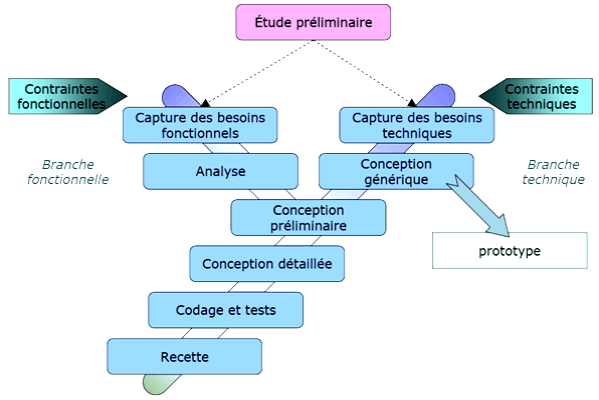
\includegraphics{./figure/illustrationDeveloppementEnY.png}
  \caption{Illustration du processus de développement en Y}
\end{figure}


% \begin{figure}[htbp]
%   \begin{tikzpicture}[node distance=2cm]
%     \tikzstyle{startstop} = [rectangle, rounded corners, minimum width=3cm, minimum height=1cm,text centered, draw=black, fill=gray!30]
%     \tikzstyle{process} = [rectangle, minimum width=3cm, minimum height=1cm, text centered, draw=black, fill=gray!10]
%     \tikzstyle{arrow} = [thick,->,>=stealth]
%     \tikzstyle{textblock} = [rectangle, text width=3cm, text centered]
%
%     % Nodes
%     \node (prelim) [startstop] {Étude préliminaire};
%     \node (functional) [textblock, left=2cm of prelim] {Contraintes fonctionnelles};
%     \node (technical) [textblock, right=2cm of prelim] {Contraintes techniques};
%     \node (funcReq) [process, below left=of prelim] {Capture des besoins fonctionnels};
%     \node (techReq) [process, below right=of prelim] {Capture des besoins techniques};
%     \node (analysis) [process, below=of funcReq] {Analyse};
%     \node (genericDesign) [process, below=of techReq] {Conception générique};
%     \node (prelimDesign) [process, below=of analysis, xshift=2cm] {Conception préliminaire};
%     \node (detailedDesign) [process, below=of prelimDesign] {Conception détaillée};
%     \node (coding) [process, below=of detailedDesign] {Codage et tests};
%     \node (testing) [process, below=of coding] {Recette};
%     \node (prototype) [process, right=of genericDesign, xshift=1cm] {Prototype};
%
%     % Arrows
%     \draw [arrow] (prelim) -- (funcReq);
%     \draw [arrow] (prelim) -- (techReq);
%     \draw [arrow] (funcReq) -- (analysis);
%     \draw [arrow] (techReq) -- (genericDesign);
%     \draw [arrow] (analysis) -- (prelimDesign);
%     \draw [arrow] (genericDesign) -- (prelimDesign);
%     \draw [arrow] (prelimDesign) -- (detailedDesign);
%     \draw [arrow] (detailedDesign) -- (coding);
%     \draw [arrow] (coding) -- (testing);
%     \draw [arrow] (genericDesign) -- (prototype);
%
%     % Text blocks
%     \node at (-3.5, -1) [textblock] {Branche fonctionnelle};
%     \node at ( 4.5, -1) [textblock] {Branche technique};
%
%   \end{tikzpicture}
%
% \end{figure}



\subsubsection{2TUP et UML}
L’utilisation de l’UML est étroitement liée au 2TUP. Les différents types de
diagrammes UML (diagramme de cas d’utilisation, de classes, de séquence et d’état)
sont largement utilisés tout au long du processus de développement pour modéliser
et documenter les besoins, les architectures, les interactions et les comportements
du système logiciel en cours de développement. L’UML fournit un langage visuel
standard et universellement accepté pour la représentation des systèmes logiciels.
Cela facilite la communication et la collaboration entre les membres de l’équipe
de développement et les
parties prenantes du projet.


\chapter{Analyse et conception}
Ce chapitre se concentre sur l’analyse approfondie des besoins de la plateforme
web et mobile pour la création collaborative et le partage d’arbres généalogiques
à \firm. Il présente également la conception de cette plateforme. L’analyse
approfondie des besoins est une étape importante dans le processus de développement,
car elle permet de définir clairement les fonctionnalités et les exigences
techniques nécessaires à la réalisation du projet. La conception, quant à elle,
vise à traduire ces besoins en solutions techniques efficaces et robustes.
Ce chapitre présentera donc en détail les besoins fonctionnels et techniques
identifiés lors de l’analyse, donnant ainsi les bases solides pour la conception de la plateforme.


\section{Analyse du besoin}
L'analyse du besoin vise à comprendre en profondeur les attentes et les exigences
des utilisateurs ainsi que les contraintes techniques et fonctionnelles qui
guideront le développement de la plateforme. Cette analyse repose sur une
étude approfondie des besoins fonctionnels et techniques.

\subsection{Besoins fonctionnels}
Les besoins fonctionnels définissent les fonctionnalités et les services que la
plateforme doit fournir à ses utilisateurs. Ils sont étroitement liés aux
objectifs et aux cas d’usage du système. Ces besoins incluent :

\begin{itemize}

  \item Création et gestion d’arbres généalogiques : les utilisateurs enregistrés
    peuvent créer, modifier et supprimer des arbres généalogiques et gérer les
    informations sur leurs proches;

  \item Consultation des arbres existants : les utilisateurs doivent pouvoir
    consulter les arbres généalogiques disponibles, y compris les détails sur
    les membres de leur famille;

  \item Recherche de membres de la famille : les utilisateurs doivent pouvoir
    trouver des personnes dans les arbres généalogiques existants sans avoir à
    créer de compte;

  \item Collaboration entre utilisateurs sur le même arbre : les utilisateurs
    enregistrés doivent pouvoir collaborer à la création et à la gestion d’un
    arbre généalogique, en y ajoutant, modifiant ou supprimant des informations
    sur les membres de la famille;

  \item Gestion des droits d’accès et de confidentialité : les utilisateurs doivent
    pouvoir déterminer qui aura accès aux arbres généalogiques qu’ils ont créés et
    gérés. Ils peuvent ainsi contrôler qui peut consulter, modifier ou contribuer
    aux informations contenues dans l’arbre;

  \item Partage et diffusion des arbres : les utilisateurs doivent pouvoir partager
    leurs arbres généalogiques avec leur famille et leurs proches.
    Ceux-ci auront alors accès à des versions consultables et visualisables.

\end{itemize}

\subsection{Besoins techniques}
Les besoins techniques décrivent les contraintes et les exigences liées à l’infrastructure
et aux technologies utilisées pour développer la plateforme. Cela inclut :

\begin{itemize}
  \item \textbf{Le choix des technologies de développement :} les langages de
    programmation, les frameworks et les outils qui seront utilisés pour créer
    la plateforme. Dans notre cas, nous utilisons :
    \begin{itemize}
      \item Langage de programmation : TypeScript (web et mobile)
      \item Frameworks : Next.js (web), Expo (mobile)
    \end{itemize}

  \item \textbf{La gestion des données :} la manière dont les informations sur les
    arbres généalogiques et les membres de la famille seront stockées, gérées
    et sécurisées. Les données sont stockées dans une base de données
    PostgreSQL. Prisma est utilisé pour gérer les opérations de base de
    données, assurant l'intégrité et la sécurité des données grâce à des
    schémas stricts et des migrations contrôlées. Et Docker est utilisé pour
    créer un conteneurs pour le \ac{SGBD};

  \item \textbf{L’interface utilisateur :} la conception de l’interface utilisateur
    pour garantir une expérience utilisateur intuitive et conviviale.
    Next.js est utilisé pour le rendu côté serveur et les pages réactives,
    assurant une performance élevée et une expérience utilisateur fluide;

  \item \textbf{La compatibilité et la sécurité :} la compatibilité avec les navigateurs
    web et les appareils mobiles, la sécurité des données, la scalabilité pour
    gérer un grand nombre d’utilisateurs, ainsi que l’interopérabilité avec
    d’autres systèmes et services existants. Les pages et composants sont
    testés pour être compatibles avec les principaux navigateurs
    (Chrome, Firefox, Safari) et optimisés pour les appareils mobiles. Docker
    permet de facilement scaler l'application pour gérer une augmentation du
    nombre d'utilisateurs. Les mesures de sécurité incluent l'utilisation de
    HTTPS, la gestion des sessions sécurisées, et des pratiques de développement
    sécurisées pour éviter les vulnérabilités courantes;

  \item \textbf{La gestion des erreurs :} la gestion des erreurs et des exceptions
    pour garantir la fiabilité et la robustesse de la plateforme. Les erreurs
    sont gérées de manière élégante et informative pour les utilisateurs, tout
    en étant enregistrées et surveillées pour permettre une résolution rapide
    des problèmes.

\end{itemize}

\section{Conception du système}
Dans cette section, nous aborderons les spécifications fonctionnelles du
système. Nous décrirons les acteurs impliqués, les cas d’utilisation identifiés,
ainsi que les relations et la classification de ces cas d’utilisation.

\subsection{Spécifications fonctionnelles}
Les spécifications fonctionnelles décrivent les fonctionnalités et les interactions
du système avec ses utilisateurs. Elles fournissent une vue détaillée des
besoins opérationnels du système.

\subsubsection{Identification des acteurs}
Les acteurs sont les entités externes qui interagissent avec le système.
Dans notre plateforme de création collaborative et de partage d'arbres
généalogiques à Mazala-Firm, les acteurs identifiés comprennent :

\begin{itemize}
  \item les membres;

  \item les administrateurs;

  \item et les visiteurs.

\end{itemize}

\subsubsection{Diagramme de contexte statique}
Le diagramme de contexte statique représente graphiquement les acteurs et leurs
relations avec le système. Il fournit une vue d’ensemble claire des interactions
entre les différentes entités impliquées dans notre plateforme de création
collaborative et de partage d’arbres généalogiques. Ce diagramme met en évidence
les liens essentiels entre les utilisateurs inscrits, les administrateurs du
système et les visiteurs non enregistrés, ce qui illustre la dynamique de
notre écosystème numérique.

\begin{figure}[htbp]
  \centering
  \begin{tikzpicture}[node distance=2cm, every node/.style={inner sep=3pt}]
    \node (system) [draw, rectangle, minimum width=2.5cm, text width=2cm, align=center] {Système};
    \node (utilisateurs) [above left=of system] {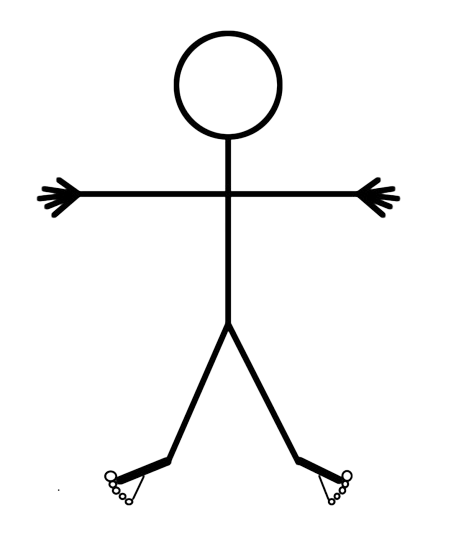
\includegraphics[width=1cm]{images/stickman.png}};
    \node (admins) [above right=of system] {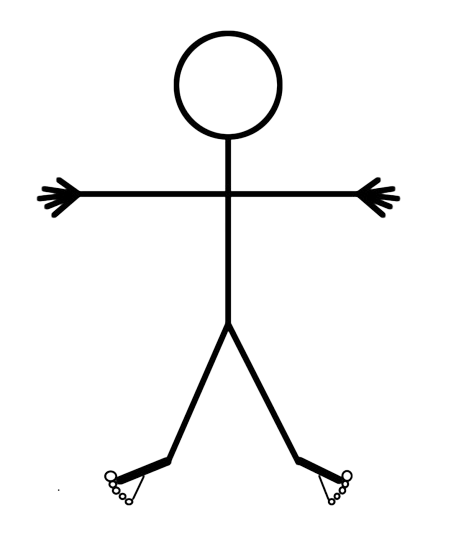
\includegraphics[width=1cm]{images/stickman.png}};
    \node (visiteurs) [below=of system] {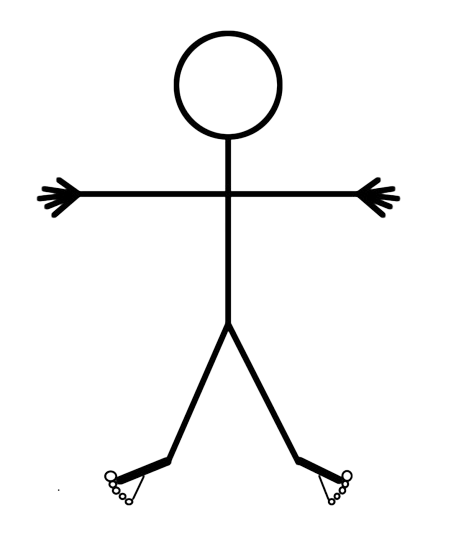
\includegraphics[width=1cm]{images/stickman.png}};

    \draw[->] (utilisateurs) -- node[anchor=south] {1..*} (system);
    \draw[->] (admins) -- node[anchor=east] {1..*} (system);
    \draw[->] (visiteurs) -- node[anchor=east] {1..*} (system);

    \node[right=0.3cm of utilisateurs] {Membre};
    \node[right=0.3cm of admins] {Administrateurs};
    \node[right=0.3cm of visiteurs] {Visiteurs};
  \end{tikzpicture}
  \caption{Diagramme de contexte statique}
\end{figure}


\subsubsection{Identification des cas d'utilisation}
Les cas d'utilisation décrivent les interactions entre les acteurs et le
système afin atteindre des objectifs spécifiques. Pour notre sytème, on retouve :

\begin{itemize}
  \item Gérer un arbre généalogique;

  \item Gérer des membres;

  \item Modifier les informations des membres;

  \item Consulter un arbre généalogique;

  \item Rechercher des membres de la famille;

  \item Accorder des droits d'accès et de confidentialité;

  \item Partager un arbre généalogique;

  \item Collaborer à la création d'un arbre généalogique;

  \item Gérer un profile;

  \item Administrer le système.

\end{itemize}


\subsubsection{Relation entre les cas d'utilisation (Use case)}
Pour affiner la représentation des interactions entre les différents cas
d’utilisation de notre système, nous utilisons les relations standardisées
définies par UML. Ces relations permettent de mieux comprendre les liens entre
les différentes fonctionnalités du système. Voici comment elles s’appliquent
dans notre contexte :

\begin{itemize}

  \item Inclusion (\say{include}) : cette relation est utilisée lorsqu’un cas
    d’utilisation de base incorpore explicitement un autre cas d’utilisation,
    de manière obligatoire. Dans notre système, nous pourrions par exemple
    inclure le cas d’utilisation \say {Modifier les informations des membres}
    dans le cas d’utilisation \say{Gérer des membres}, car la modification des
    informations des membres fait partie intégrante de la gestion des membres.

  \item Extension (\say{extend}) : cette relation est utilisée lorsqu’une
    utilisation de base incorpore implicitement un autre cas d’utilisation, de
    façon optionnelle. Par exemple, le cas d’utilisation \say{Partager un arbre généalogique}
    peut être étendu par le cas d’utilisation \say{Accorder des droits d’accès et de confidentialité}.
    Ainsi, lorsqu’un utilisateur souhaite partager un arbre généalogique, il a
    également la possibilité d’accorder des droits d’accès spécifiques à
    certains membres de sa famille.

  \item Généralisation/spécialisation : cette relation sert à décrire un lien
    du genre \say{est un} entre différents cas d’utilisation. Dans notre système,
    on peut trouver une généralisation entre les cas d’utilisation \say {Gérer un
    arbre généalogique} et \say{Gérer des membres}, puisque gérer un arbre
    généalogique inclut aussi la gestion des membres qui en font partie. Les
    fonctionnalités de gestion des membres peuvent donc être considérées comme
    une spécialisation du cas d’utilisation de gestion d’un arbre généalogique.

\end{itemize}


\newpage
\begin{figure}
  \begin{tikzpicture}

% Actors
\umlactor[x=-3, y=3]{Visiteur}
\umlactor[x=-3, y=1]{Membre}
\umlactor[x=-3, y=-2]{Admin}

% Use Cases
\begin{umlsystem}[x=0, y=0, fill=white]{Plateforme Mazala-Firm}
  \umlusecase[x=0, y=4]{Consulter arbre}
  \umlusecase[x=0, y=2]{Rechercher membres}
  \umlusecase[x=0, y=0]{Partager arbre}
  \umlusecase[x=5, y=4]{Gérer arbre}
  \umlusecase[x=5, y=2]{Gérer membres}
  \umlusecase[x=5, y=0]{Modifier infos}
  \umlusecase[x=10, y=4]{Collaborer arbre}
  \umlusecase[x=10, y=2]{Accorder droits}
  \umlusecase[x=10, y=0]{Gérer profil}
  \umlusecase[x=10, y=-2]{Administrer}
\end{umlsystem}

% Associations
\umlassoc{Visiteur}{usecase-1}
\umlassoc{Visiteur}{usecase-2}
\umlassoc{Membre}{usecase-3}
\umlassoc{Membre}{usecase-4}
\umlassoc{Membre}{usecase-5}
\umlassoc{Membre}{usecase-6}
\umlassoc{Membre}{usecase-7}
\umlassoc{Membre}{usecase-8}
\umlassoc{Membre}{usecase-9}
\umlassoc{Admin}{usecase-10}

% Relationships
\umlinclude{usecase-4}{usecase-5}
\umlinclude{usecase-5}{usecase-6}
\umlVHextend{usecase-3}{usecase-8}
\umlinherit{usecase-5}{usecase-4}

\end{tikzpicture}
  \caption{Diagramme de cas d'utilisation}
\end{figure}

\subsubsection{Classification des cas d'utilisation (priorités, risques et itérations)}
Dans cette section, nous classons les cas d’utilisation identifiés selon leur
priorité, leur niveau de risque et leur inclusion dans les itérations du
développement. Cette classification servira à guider la planification et
l’exécution du projet en mettant en évidence les fonctionnalités les plus
importantes, les risques potentiels à surveiller et les étapes itératives du
développement.

\begin{table}[htbp]
  \centering
  \begin{tabularx}{\textwidth}{|l|l|l|X|}
    \hline
    \textbf{Cas d'utilisation} & \textbf{Priorité} & \textbf{Risque} & \textbf{Itération} \\ \hline
    Gérer un arbre généalogique & Forte & Moyen & 1 \\ \hline
    Gérer des membres & Forte & Moyen & 1 \\ \hline
    Modifier les informations des membres & Moyenne & Faible & 1 \\ \hline
    Consulter un arbre généalogique & Forte & Faible & 1 \\ \hline
    Rechercher des membres de la famille & Moyenne & Moyen & 2 \\ \hline
    Accorder des droits d’accès et de confidentialité & Moyenne & Élevé & 2 \\ \hline
    Partager un arbre généalogique & Forte & Élevé & 2 \\ \hline
    Collaborer à la création d’un arbre généalogique & Forte & Élevé & 3 \\ \hline
    Gérer un profil & Moyenne & Moyen & 3 \\ \hline
    Administrer le système & Moyenne & Élevé & 3 \\ \hline
  \end{tabularx}
  \caption{Classification des cas d'utilisation en fonction de la priorité, du risque et de l'itération}
\end{table}

Dans le tableau ci-dessus, chaque cas d’utilisation est évalué selon trois critères principaux :

\begin{itemize}

  \item Priorité : indique l’importance relative du cas d’utilisation pour
    l’achèvement du projet. Les priorités peuvent être classées comme forte, moyennes ou basses.

  \item Risque : évalue le niveau de risque associé à la mise en œuvre du cas
    d’utilisation. Les risques peuvent être classés comme faibles, moyens ou élevés.

  \item Itération : indique dans quelle itération du développement le cas
    d’utilisation sera implémenté. Les itérations peuvent être numérotées séquentiellement.

\end{itemize}

Cette classification constituera un outil précieux pour la planification et la
gestion du projet. Elle permettra une allocation efficace des ressources et
une identification proactive des risques potentiels.

\newpage

\subsection{Spécification détaillée }
Dans cette section, nous fournissons une spécification détaillée des cas
d’utilisation identifiés. Nous décrivons les interactions entre les acteurs et
le système, ainsi que les flux d’événements associés.

\subsubsection{Description textuelle d'un cas d'utilisation}
\textbf{Cas d’utilisation :} Gérer un arbre généalogique

\textbf{Acteur :} Utilisateur enregistré

\textbf{Autres acteurs :} Système

\textbf{Description :} Ce cas d’utilisation permet à l’utilisateur de créer,
de modifier, de visualiser et de supprimer des arbres généalogiques.

\textbf{Préconditions :} L’utilisateur est authentifié et peut accéder à la
fonctionnalité de gestion des arbres généalogiques.

\textbf{Postconditions :} Les modifications apportées à l'arbre généalogique
sont enregistrées dans le système.

\textbf{Séquencement des événements}

Le cas d’utilisation commence lorsque l’utilisateur se connecte à la plateforme
et desire gérer un arbre généalogique.

\textbf{Scénario nominal :}

\begin{enumerate}

  \item  L’utilisateur se connecte à l’application.

  \item Le système affiche alors une barre de navigation latérale comportant un
    bouton \say{Créer un arbre} ainsi qu’une liste d’arbres généalogiques déjà
    existants chez cet utilisateur.

  \item L’utilisateur peut ensuite sélectionner parmi les options suivantes :
    \begin{itemize}
      \item Créer un nouvel arbre généalogique;
      \item Modifier un arbre généalogique existant;
      \item Consulter un arbre généalogique existant;
      \item Supprimer un arbre généalogique existant;
      \item Visualiser un arbre généalogique existant.
    \end{itemize}

  \item Si l’utilisateur décide de créer un nouvel arbre généalogique :
    \begin{enumerate}
      \item il doit cliquer sur le bouton \say{Créer un nouvel arbre};
      \item le système affiche une fenêtre où il devra entrer un nom et un type(publique, privé)
        pour son nouvel arbre généalogique;
      \item l’utilisateur valide ses informations;
      \item le système crée alors un nouvel arbre généalogique et l’affiche dans la liste des arbres
        généalogiques de l’utilisateur.
    \end{enumerate}

  \item  Si l’utilisateur décide de modifier un arbre généalogique existant :
    \begin{enumerate}
      \item il sélectionne l’arbre généalogique dans la barre de navigation latérale.;
      \item le système affiche alors les détails de l’arbre généalogique sélectionné;
      \item utilisateur effectue les modifications nécessaires (ajouts,
        suppressions, modifications de membres ou de relations) ou les
        informations de l’arbre généalogique;

        \subitem Pour ajouter un membre :

          \begin{itemize}
            \item l’utilisateur clique sur l’option \say{Ajouter un membre};
            \item le e système présente un formulaire qui demande des
              renseignements au sujet du nouveau membre (son nom, sa date de
              naissance, ses relations, etc.);
            \item l’utilisateur remplit les champs requis et valide son entrée;
            \item le système ajoute le nouveau membre à l’arbre généalogique;
          \end{itemize}

        \subitem Pour modifier les informations de l’arbre généalogique :

          \begin{itemize}
            \item l’utilisateur clique sur l’option \say{Modifier les informations};
            \item le système affiche un formulaire de modification des informations de l’arbre généalogique;
            \item l’utilisateur effectue les modifications nécessaires et valide ses changements;
            \item le système enregistre les modifications apportées à l’arbre généalogique.
          \end{itemize}

      \item le système sauvegarde toutes les modifications apportées à l’arbre généalogique.
    \end{enumerate}

  \item Si l’utilisateur souhaite consulter, un arbre généalogique existant :
    \begin{enumerate}
      \item il sélectionne l’arbre généalogique dans la barre de navigation latérale;
      \item le système affiche alors l’arbre généalogique sélectionné avec les
        informations sur ses membres et leurs liens.
    \end{enumerate}

  \item Si l’utilisateur souhaite supprimer un arbre généalogique existant :
    \begin{enumerate}
      \item il sélectionne l’arbre généalogique dans la barre de navigation latérale;
      \item le système demande une confirmation avant de procéder à la
        suppression définitive de l’arbre généalogique;
      \item si l’utilisateur accepte, le système efface l’arbre généalogique
        ainsi que toutes les données connexes de la liste dans la barre de
        navigation latérale.
    \end{enumerate}

\end{enumerate}

\textbf{Scénario alternatif :}

\subsubsection*{Scénarios alternatifs}

\begin{enumerate}
    \item \textbf{Scénario alternatif pour la création d'un arbre généalogique :}
    \begin{itemize}
        \item \textbf{Étape 4a :} L'utilisateur tente de créer un arbre
          généalogique mais ne saisit pas un nom valide ou ne choisit pas un type.
        \begin{itemize}
            \item le système affiche un message d'erreur demandant de saisir
              un nom valide ou de choisir un type;
            \item l'utilisateur saisit un nom valide ou choisit un type et confirme;
            \item Le système crée le nouvel arbre généalogique et l'ajoute à la liste.
        \end{itemize}
    \end{itemize}

    \item \textbf{Scénario alternatif pour la modification d'un arbre généalogique :}
    \begin{itemize}
        \item \textbf{Étape 5a :} L'utilisateur tente d'ajouter un membre mais
          laisse des champs obligatoires vides.
        \begin{itemize}
            \item le système affiche un message d'erreur demandant de compléter les champs obligatoires;
            \item l'utilisateur complète les informations manquantes et confirme;
            \item le système ajoute le nouveau membre à l'arbre généalogique.
        \end{itemize}
    \end{itemize}

    \item \textbf{Scénario alternatif pour la suppression d'un arbre généalogique :}
    \begin{itemize}
        \item \textbf{Étape 7a :} L'utilisateur sélectionne un arbre généalogique à supprimer mais change d'avis et annule l'opération.
        \begin{itemize}
            \item Le système annule l'opération de suppression et revient à la liste des arbres généalogiques.
        \end{itemize}
    \end{itemize}

    \item \textbf{Scénario alternatif pour la visualisation d'un arbre généalogique :}
    \begin{itemize}
        \item \textbf{Étape 6a :} L'utilisateur tente de visualiser un arbre
          généalogique mais celui-ci contient des erreurs de données (ex. : relations incorrectes).
        \begin{itemize}
            \item le système affiche un message d'erreur et propose des options de correction.
            \item l'utilisateur corrige les erreurs et le système affiche l'arbre généalogique mis à jour.
        \end{itemize}
    \end{itemize}

\end{enumerate}

\textbf{Scénario d'exception :}
\begin{enumerate}
  \item Si, à l’étape 3, l’utilisateur ferme la barre de navigation latérale
    ,le scénario principal est interrompu.

  \item Si l’utilisateur essaie de supprimer un arbre généalogique sans avoir
    obtenu de confirmation, le système annule
\end{enumerate}

Cette description textuelle fournit une vue détaillée des étapes et des
interactions impliquées dans le cas d’utilisation \say{Gérer un arbre généalogique}.
Cela permet une compréhension claire des fonctionnalités offertes par ce cas
d’utilisation.


\subsubsection{Diagramme de séquence}

Le diagramme de séquence est un outil visuel permettant de représenter les
interactions entre les acteurs et le système dans un scénario donné. Il montre
la séquence des messages échangés entre les objets du système au cours d’un
scénario d’exécution. Dans notre cas, nous allons illustrer le scénario de
création et de suppression d’un arbre généalogique par un utilisateur.



\begin{center}
  \newpage
  \textbf{Gestion d'un arbre généalogique}

  \begin{figure}[htbp]
    \centering
    \begin{sequencediagram}

      \newthread{user}{Utilisateur}
      \newinst[7]{sys}{Système}  % Adjusting the distance here

      \begin{sdblock}{Connexion}{}
        \begin{call}{user}{Se connecter}{sys}{Page de connexion}
          \mess{sys}{Afficher page de connexion}{user}
          \begin{call}{user}{Entrer identifiants}{sys}{Authentifier}
            \mess{sys}{Valider identifiants}{user}
          \end{call}
        \end{call}
      \end{sdblock}

      \begin{sdblock}{Opérations sur Arbre Généalogique}{}
        \begin{call}{user}{Sélectionner une action CRUD}{sys}{Afficher page correspondante}
          \begin{call}{user}{Entrer ou confirmer les détails}{sys}{Valider l'opération}
            \mess{sys}{Mettre à jour la base de données et afficher le résultat}{user}
          \end{call}
        \end{call}
      \end{sdblock}

    \end{sequencediagram}

    \caption{Diagramme de séquence pour gestion d'un arbre généalogique}
  \end{figure}

\end{center}

\subsubsection{Diagramme d'activité}

Le diagramme d’activité est un outil visuel qui permet de représenter le flux
de contrôle entre les différentes activités d’un système. Il montre comment les
activités sont organisées et enchaînées pour atteindre un objectif spécifique.
Dans notre cas, nous allons illustrer le processus d’ajout d’un membre à un
arbre de la famille dans un arbre généalogique.
% \tikzstyle{startstop} = [rectangle, rounded corners, minimum width=3cm, minimum height=1cm, text centered, draw=black, fill=red!30]
% \tikzstyle{process} = [rectangle, minimum width=3cm, minimum height=1cm, text centered, draw=black, fill=orange!30]
% \tikzstyle{decision} = [diamond, minimum width=3cm, minimum height=1cm, text centered, draw=black, fill=green!30]
% \tikzstyle{arrow} = [thick,->,>=stealth]

% \tikzstyle{startstop} = [draw, circle, rounded corners, minimum width=1cm, minimum height=1cm, text centered, draw=black]
% \tikzstyle{process} = [rectangle, minimum width=3cm, minimum height=1cm, text centered, draw=black]
% \tikzstyle{decision} = [diamond, minimum width=3cm, minimum height=1cm, text centered, draw=black]
% \tikzstyle{arrow} = [thick,->,>=stealth]


\begin{figure}[htbp]
  \centering
  \tikzstyle{startstop} = [draw, circle, fill=black, text=white, minimum width=1cm, minimum height=1cm, text centered, draw=black]
  \tikzstyle{stop} = [draw, circle, minimum width=1cm, minimum height=1cm, text centered, draw=black, path picture={
    \draw[black, thick] (path picture bounding box.south west) -- (path picture bounding box.north east);
    \draw[black, thick] (path picture bounding box.north west) -- (path picture bounding box.south east);
  }]
  \tikzstyle{process} = [rectangle, minimum width=3cm, minimum height=1cm, text centered, draw=black]
  \tikzstyle{decision} = [diamond, minimum width=1cm, minimum height=1cm, text centered, draw=black]
  \tikzstyle{arrow} = [thick,->,>=stealth]
  \begin{tikzpicture}[node distance=2cm]

    \node (start) [startstop] {Début};
    \node (login) [process, below of=start] {Se connecter};
    \node (displayNav) [process, below of=login] {Afficher barre de navigation};
    \node (selectTree) [decision, below of=displayNav] {};
    \node (firstStop) [startstop, right=3cm of selectTree] {Fin};
    \node (fillForm) [process, below of=selectTree, yshift=-1cm] {Entrer ou confirmer les détails};
    \node (validate) [decision, below of=fillForm, yshift=-1cm] {};
    \node (saveMember) [process, below of=validate, yshift=-1cm] {Sauvegarder le membre};
    \node (stop) [startstop, below of=saveMember] {Fin};

    \draw [arrow] (start) -- (login);
    \draw [arrow] (login) -- (displayNav);
    \draw [arrow] (displayNav) -- (selectTree);
    \draw [arrow] (selectTree) -- node[anchor=east] {Oui} (fillForm);
    \draw [arrow] (selectTree) -- node[anchor=south] {Non} (firstStop);
    \draw [arrow] (fillForm) -- (validate);
    \draw [arrow] (validate) -- node[anchor=east] {Oui} (saveMember);
    \draw [arrow] (saveMember) -- (stop);
    \draw [arrow] (validate.east) -- ++(3,0) |- node[anchor=center] {Non} (firstStop);

    \node[left=0.3cm of selectTree] {Choix d'une action};
    \node[left=0.3cm of selectTree] {Choix d'une action};
    \node[left=0.3cm of validate] {Validate ?};

  \end{tikzpicture}
  \caption{Diagramme d'activité pour la gestion d'un arbre généalogique}
\end{figure}


\newpage
\subsection{Réalisations des cas d'utilisation}
Dans cette section, nous abordons la mise en œuvre concrète des cas
d’utilisation identifiés précédemment. À ce stade, nous traduisons les
interactions entre les acteurs et le système en fonctionnalités opérationnelles.
Nous détaillons également les règles de gestion spécifiques qui guident le
comportement du système lors de l’exécution de chaque cas d’utilisation. Enfin,
nous présentons le modèle du domaine sous forme d’un diagramme de classe du
système, offrant ainsi une vue structurée des entités et de leurs relations
au sein du système.
\subsubsection{Quelques règles de gestion}

Nous allons établir ici un ensemble de règles de gestion qui régissent le
comportement des fonctionnalités mises en œuvre. Ces règles définissent les
contraintes et les conditions d’exécution pour garantir la cohérence et la
fiabilité des opérations réalisées par le système.

\begin{itemize}
  \item \textbf{Règle de gestion 1 :} Un utilisateur ne peut pas modifier un arbre généalogique qui ne lui appartient pas.
  \item \textbf{Règle de gestion 2 :} Un arbre généalogique ne peut pas être partagé avec des utilisateurs non enregistrés.
  \item \textbf{Règle de gestion 3 :} Un arbre généalogique privé ne peut être consulté que par son propriétaire.
  \item \textbf{Règle de gestion 4 :} Un arbre généalogique publique peut être consulté par tous les utilisateurs enregistrés.
  \item \textbf{Règle de gestion 5 :} Un arbre généalogique ne peut pas être supprimé s’il contient des membres.
  \item \textbf{Règle de gestion 6 :} Un arbre généalogique ne peut pas être partagé avec des utilisateurs qui n’ont pas de compte.
\end{itemize}

\subsubsection{Modele du domaine (Diagramme de classe du système)}
Le diagramme de classe du système est une représentation visuelle des
entités principales du domaine et de leurs relations. Il offre une vue
d'ensemble de la structure du système, en mettant en évidence les différentes
classes d'objets, leurs attributs et leurs associations. Cette représentation
facilite la compréhension des concepts clés du domaine et guide la conception
de la solution logicielle.


\newpage
\begin{figure}[htbp]
  \begin{tikzpicture}

    % User class
    \umlclass{Utilisateur}{
      + id : String \\
      + nomUtilisateur : String \\
      + email : String \\
      + MdpHaché : String \\
      + DateCreation : DateTime \\
      + DateModifier : DateTime
    }{
      + créerArbre() : void \\
      + modifierArbre() : void \\
      + supprimerArbre() : void \\
      + visualiserArbre() : void
    }

    % Profile class
    \umlclass[x=0, y=-6]{Profil}{
      + id : String \\
      + prénom : String \\
      + nom : String \\
      + avatarURL : String
    }{}

    % UserAccess class
    \umlclass[x=7, y=-5]{AccèsUtilisateur}{
      + id : String \\
      + level : NiveauAccès \\
      + userExternalId : String \\
      + treeId : String
    }{}

    % Tree class
    \umlclass[x=7, y=-10]{Arbre}{
      + id : String \\
      + name : String \\
      + type : TypeArbre
    }{
      + ajouterMembre() : void \\
      + modifierMembre() : void \\
      + supprimerMembre() : void
    }

    % Member class
    \umlclass[x=0, y=-10]{Membre}{
      + id : String \\
      + firstname : String \\
      + nom : String \\
      + dateNaissance : DateTime \\
      + lieuNaissance : String \\
      + sexe : Sexe \\
      + avatarURL : String \\
      + description : String
    }{}

    % Relation class
    \umlclass[x=0, y=-16]{Relation}{
      + idPapa : String \\
      + idMaman : String \\
      + conjoints : String[] \\
      + enfants : String[] \\
      + idMembre : String
    }{}

    % Enums
    \umlenum[x=14, y=-5]{NiveauAccès}{
      admin \\
      editeur \\
      lecteur
    }

    \umlenum[x=14, y=-10]{TypeArbre}{
      publique \\
      privé
    }

    \umlenum[x=14, y=-15]{Sexe}{
      masculin \\
      feminin
    }

    % Aggregations and Compositions
    \umluniaggreg[mult1=1, pos1=0.7, mult2=0..1, pos2=0.3]{Utilisateur}{Profil}
    \umluniaggreg[mult1=1, pos1=0.7, mult2=*, pos2=0.3]{Utilisateur}{AccèsUtilisateur}
    \umluniaggreg[mult1=1, pos1=0.7, mult2=*, pos2=0.3]{Arbre}{Membre}
    \umluniaggreg[mult1=1, pos1=0.7, mult2=*, pos2=0.3]{Arbre}{AccèsUtilisateur}
    \umlunicompo[mult1=1, pos1=0.7, mult2=0..1, pos2=0.3]{Membre}{Relation}

    % Relationships
    \umluniassoc[mult1=1, pos1=0.7, mult2=1, pos2=0.3]{Profil}{Utilisateur}
    \umluniassoc[mult1=1, pos1=0.7, mult2=*, pos2=0.3]{AccèsUtilisateur}{Utilisateur}
    \umluniassoc[mult1=1, pos1=0.7, mult2=*, pos2=0.3]{AccèsUtilisateur}{Arbre}
    \umluniassoc[mult1=1, pos1=0.7, mult2=*, pos2=0.3]{Membre}{Arbre}
    \umluniassoc[mult1=1, pos1=0.7, mult2=1, pos2=0.3]{Relation}{Membre}

    % Enum Relations
    \umluniassoc[mult1=1, pos1=0.7, mult2=*, pos2=0.3]{AccèsUtilisateur}{NiveauAccès}
    \umluniassoc[mult1=1, pos1=0.7, mult2=*, pos2=0.3]{Arbre}{TypeArbre}
    \umluniassoc[mult1=1, pos1=0.7, mult2=*, pos2=0.3]{Membre}{Sexe}

  \end{tikzpicture}
  \caption{Diagramme de classe du système}
\end{figure}


\subsubsection{Diagramme d'objet}
Un diagramme d’objet représente graphiquement les objets et leurs relations à
un moment donné. À l’inverse du diagramme de classe, qui décrit la structure
statique des classes et de leurs relations dans un système, le diagramme
d’objet illustre des instances spécifiques des classes (objets) et les liens
entre eux dans un contexte particulier. Il est utilisé pour visualiser l’état
d’un système à un instant précis, facilitant la compréhension des interactions
dynamiques et des configurations temporaires des objets.

\begin{figure}[htbp]
    \centering
    \begin{tikzpicture}[
        object/.style={rectangle, draw, text width=6cm, minimum height=1cm, align=left, font=\ttfamily},
        attribute/.style={text width=7cm, align=left, font=\ttfamily}
    ]

        % Object instances
        \node[object] (utilisateur1) {
            \textbf{Utilisateur: utilisateur1} \\
            \underline{id} = "u1234" \\
            \underline{nomUtilisateur} = "jdoe" \\
            \underline{email} = "jdoe@example.com" \\
            \underline{MdpHaché} = "******" \\
            \underline{DateCreation} = "2022-01-01" \\
            \underline{DateModifier} = "2022-02-01"
        };

        \node[object, below=of utilisateur1] (profile1) {
            \textbf{Profil: profile1} \\
            \underline{id} = "p1234" \\
            \underline{prénom} = "John" \\
            \underline{nom} = "Doe" \\
            \underline{avatarURL} = "http://example.com/avatar.jpg"
        };

        \node[object, right=of utilisateur1] (acces1) {
            \textbf{AccèsUtilisateur: acces1} \\
            \underline{id} = "a1234" \\
            \underline{level} = "admin" \\
            \underline{userExternalId} = "u1234" \\
            \underline{treeId} = "t1234"
        };

        \node[object, below=of acces1] (arbre1) {
            \textbf{Arbre: arbre1} \\
            \underline{id} = "t1234" \\
            \underline{name} = "Doe Family Tree" \\
            \underline{type} = "privé"
        };

        \node[object, below=of profile1] (member1) {
            \textbf{Membre: member1} \\
            \underline{id} = "m1234" \\
            \underline{firstname} = "Jane" \\
            \underline{nom} = "Doe" \\
            \underline{dateNaissance} = "1990-01-01" \\
            \underline{lieuNaissance} = "Paris" \\
            \underline{sexe} = "féminin" \\
            \underline{avatarURL} = "http://example.com/jane.jpg" \\
            \underline{description} = "Daughter of John Doe"
        };

        \node[object, below=of member1] (relation1) {
            \textbf{Relation: relation1} \\
            \underline{idPapa} = "m1234" \\
            \underline{idMaman} = "m1235" \\
            \underline{conjoints} = ["m1236"] \\
            \underline{enfants} = ["m1237"] \\
            \underline{idMembre} = "m1234"
        };

        % Relationships
        \draw[->] (utilisateur1) -- (profile1);
        \draw[->] (utilisateur1) -- (acces1);
        \draw[->] (acces1) -- (arbre1);
        \draw[->] (arbre1) -- (member1);
        \draw[->] (member1) -- (relation1);

    \end{tikzpicture}
    \caption{Diagramme d'objet du système}
\end{figure}


\newpage
\subsection{Conception architecturale}
La conception architecturale est une étape importante du développement logiciel
qui vise à définir la structure globale d’un système et de ses composants
principaux. Elle comprend l’organisation des modules, la communication entre
eux et les contraintes techniques à respecter. Cette phase permet de créer une
base solide pour le développement, afin d’assurer que les exigences
fonctionnelles et non fonctionnelles seront satisfaites. La conception
architecturale se décline en plusieurs sous-sections, notamment l’architecture
logicielle et l’architecture globale de la solution.

\subsubsection{Architecture logicielle}
L’architecture logicielle décrit la structure organisationnelle d’un système
logiciel, y compris ses modules, leurs responsabilités et les interactions
entre eux. Elle vise à garantir la cohérence, la performance, la maintenabilité
et la scalabilité du système. L’architecture logicielle est un guide pour les
développeurs qui permet d’aligner les décisions techniques avec les objectifs
métier et les contraintes du projet.

Pour notre projet, nous avons opté pour une architecture basée sur plusieurs
patterns et concepts pour structurer nos applications.

\begin{itemize}
  \item \textbf{Architecture pour l'application web }

    Notre architecture se distingue par sa capacité à offrir un rendu côté
    serveur (SSR - Server-Side Rendering) ainsi que des pages statiques générées
    à la compilation (SSG - Static Site Generation). Cela améliore à la fois
    les performances et l’optimisation pour les moteurs de recherche (SEO).

    En outre, cette architecture permet de séparer les pages, les composants et
    les API, offrant ainsi une organisation plus claire et modulable.

  \item \textbf{Architecture pour l'application mobile}

    Notre architecture offre une expérience de développement simplifiée. Elle
    permet de développer des applications mobiles rapidement et efficacement grâce
    à des outils intégrés pour la gestion de la configuration, l’accès aux API
    natives, et les mises à jour en direct (OTA — Over-The-Air).

    Enfin, elle permet de séparer les vues, les composants et les services, offrant
    ainsi une organisation claire et modulaire des éléments de l’application.

    Cette approche optimise le développement cross-plateforme en utilisant une seule
    base de code pour les applications iOS et Android, tout en garantissant une
    expérience utilisateur native de haute qualité.
\end{itemize}



\subsubsection{Architecture globale de la solution (Diagramme de déploiement)}
L’architecture globale de la solution est souvent illustrée par un diagramme de
déploiement qui montre la configuration physique des composants logiciels sur
le matériel. Ce diagramme détaille comment les éléments logiciels sont
distribués à travers différents nœuds de réseau, tels que serveurs, bases de
données, et terminaux utilisateurs. Il aide à comprendre les aspects de
performance, de sécurité et de scalabilité de la solution, en montrant comment
les composants interagissent dans un environnement réel.

Dans notre cas, la plateforme pour la création collaborative et le partage
d’arbres généalogiques sont basés sur une architecture distribuée qui
comprend plusieurs composants clés.

Une architecture distribuée  désigne un système d'information ou un réseau pour
lequel l'ensemble des ressources disponibles ne se trouvent pas au même endroit
ou sur la même machine (\textcite{frwiki:212787328}).

% \begin{figure}[htbp]
%   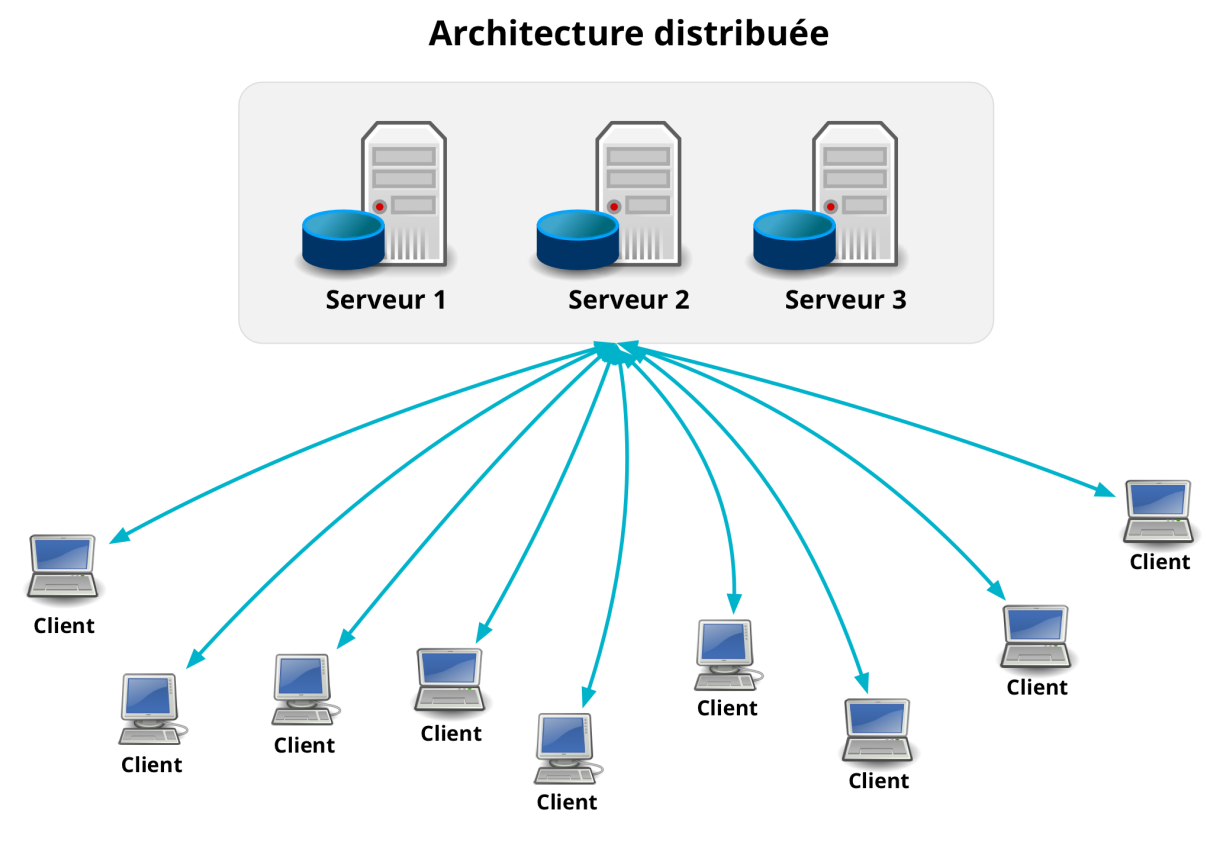
\includegraphics{images/architectureDistribuee.png}
%   \caption{Illustration de l'architecture distribuée }
% \end{figure}

\begin{itemize}
  \item \textbf{ Serveur Web :} Héberge l'application Next.js pour le rendu
    côté serveur (SSR) et le serveur API. Utilise Node.js pour exécuter le
    code JavaScript côté serveur.

  \item \textbf{Serveur de bases de données :} utilise PostgreSQL comme SGBD
    pour stocker les données relatives aux utilisateurs, aux arbres
    généalogiques et aux collaborations.

  \item \textbf{ Terminal utilisateur :} comprend les navigateurs Web pour
    accéder à l’application web Next.js et les applications mobiles Expo/React
    Native pour l’accès mobile.

  \item \textbf{Services externes :} intègre éventuellement des services
    externes pour des fonctionnalités supplémentaires, telles que
    l’authentification OAuth, le stockage de fichiers et les
    services de messagerie.

\end{itemize}

Voici un diagramme de déploiement illustrant cette architecture :

\begin{figure}[htbp]
  \centering
    \begin{tikzpicture}[
        server/.style={rectangle, draw, fill=blue!20, text centered, minimum height=2em, minimum width=4em},
        database/.style={cylinder, draw, shape border rotate=90, aspect=0.25, text centered, minimum height=2em, minimum width=4em},
        user/.style={ellipse, draw, fill=yellow!20, text centered, minimum height=2em, minimum width=4em},
        external/.style={rectangle, draw, dashed, fill=green!20, text centered, minimum height=2em, minimum width=4em},
        arrow/.style={->, thick, shorten <=2pt, shorten >=2pt}
    ]

    % Nodes
    \node[server] (webserver) {Serveur Web(Next.js/Node.js)};
    \node[database, below=of webserver, yshift=-2cm] (database) {Base de Données(PostgreSQL)};
    \node[user, left=of webserver, xshift=-1cm] (browser) {Navigateur};
    \node[user, right=of webserver, xshift=1cm] (mobileapp) {Application Mobile};
    \node[external, below=of database, yshift=-1cm] (auth) {Service d'authentification(OAuth)};

    % Arrows
    \draw[arrow] (browser) -- (webserver);
    \draw[arrow] (webserver) -- ( browser);
    \draw[arrow] (mobileapp) -- (webserver);
    \draw[arrow] (webserver) -- (mobileapp);
    \draw[arrow] (webserver) -- (database);
    \draw[arrow] (webserver) -- (auth);
    \draw[arrow] (auth) -- (webserver);

    \end{tikzpicture}
    \caption{Diagramme de déploiement}
\end{figure}

\newpage
\textbf{Avantages de cette architecture }

\begin{itemize}
  \item \textbf{Scalabilité:} les composants peuvent être mis à l’échelle
    indépendamment en fonction de la demande.

  \item \textbf{Sécurité :} la séparation des préoccupations permet
    d’améliorer la sécurité, notamment en isolant la base de données
    du reste de l’application.

  \item \textbf{Performance :} l'utilisation du rendu côté serveur et de la
    génération de pages statiques améliore la vitesse de chargement des
    pages et l’expérience utilisateur.

  \item \textbf{Maintenabilité :} l’architecture distribuée permet d’intégrer
    de nouveaux services et de mettre à jour les composants sans affecter
    l’ensemble du système.

\end{itemize}
